\documentclass[12pt,a4paper]{report}

%--------------------------------------
\usepackage[T1]{fontenc} %Not needed by LuaLaTeX or XeLaTeX
%--------------------------------------

%Portuguese-specific commands
%--------------------------------------
%\usepackage[portuguese]{babel}
%--------------------------------------

%Hyphenation rules
%--------------------------------------
\usepackage{hyphenat}
\hyphenation{mate-mática recu-perar}
%--------------------------------------

%Espaçamento e outras cenas
%--------------------------------------
\usepackage{setspace}
\usepackage{anyfontsize}
\usepackage{indentfirst}
\usepackage{parskip}
\usepackage{titlesec} % Chapter
\usepackage{geometry} % Margens
\usepackage{amsmath} % Matemática
\usepackage{graphicx}
\usepackage{wrapfig}
\usepackage{subcaption}
\usepackage{caption}
\usepackage[hidelinks]{hyperref}
\usepackage{xpatch}
\usepackage{etoolbox}
\usepackage{titletoc}
\usepackage{times}
\usepackage{fancyhdr}
\usepackage{lastpage}
%--------------------------------------

\geometry{
    a4paper,
    right = 3cm,
    left = 2.5cm,
    top = 2.5cm,
    bottom = 2.5cm,
}

\renewcommand{\contentsname}{Índice}

\setcounter{secnumdepth}{0} % Não enumerar secções

\setstretch{1.5} % espaçamento

\titleformat{\chapter}{\fontfamily{ptm}\selectfont\centering\huge\titlerule[1.5pt]\vspace{-9pt}}{}{0pt}{\Huge}[{\titlerule[1.5pt]}]

\titleformat{\section}{\bfseries\fontfamily{ptm}\selectfont}{}{0pt}{\large}[{\titlerule[1pt]}]

\titlespacing{\chapter}{0pt}{-30pt}{30pt}

\titlecontents{section}[40pt]{\vskip3pt\bfseries}{\thecontentslabel\quad}{}{~~\normalfont\dotfill\bfseries\contentspage}[]

\begin{document}

\begin{titlepage}
    \centering
    \fontsize{25}{0}\selectfont
    
    \begin{figure}
        \centering
        
\includegraphics[width=0.45\textwidth]{images/uminho.png}
        \caption*{}
        \label{fig:my_label}
    \end{figure}

    Universidade do Minho \\
    \Large Licenciatura em Engenharia Informática \\
    
    \vspace*{4.3cm}
    \Large Sistemas Operativos - Trabalho Prático \\ 
    \large Grupo 19

    \vspace*{4.3cm}
    
    \large Diogo Marques - A100897 \\
    \large Duarte Leitão - A100550 \\
    \large Gonçalo Moreira - A73591 \\

    \vspace*{1cm}

    \large 13 de maio de 2023
\end{titlepage}


\tableofcontents

\chapter{Introdução}

    No âmbito da Unidade Curricular de Sistemas Operativos foi-nos apresentado um trabalho que visa a comunicação entre um servidor e vários clientes, a fim de executar programas e apresentar estatísticas sobre os mesmos.

    Ao contrário do que seria possível depreender, neste caso os clientes são responsáveis por executar os programas que invocam, ao passo que o servidor apenas funciona como um centro estático a partir do qual os clientes podem obter informações relativas aos programas que foram executados até ao momento.

    Numa fase inicial, o maior desafio cifrou-se em perceber como deveria ser assegurada a comunicação entre os vários clientes e o servidor. Mais tarde, a execução encadeada de programas também se revelou um grande obstáculo, mas felizmente fomos capazes de ultrapassar essas dificuldades.


\chapter{Arquitetura}

    A comunicação entre o servidor e os clientes representa a parte fundamental deste projeto, já que sem isso não é possível realizar a maior parte das funcionalidades requeridas.

    \section{FIFOs Estáticos}

        A forma imediata de resolver este problema parece ser criar dois \textit{pipes} com nome (FIFOs), em que por um deles passa toda a informação destinada ao servidor, e no outro aquela que é destinada aos clientes.

        \begin{figure}[hb!]
            \centering
            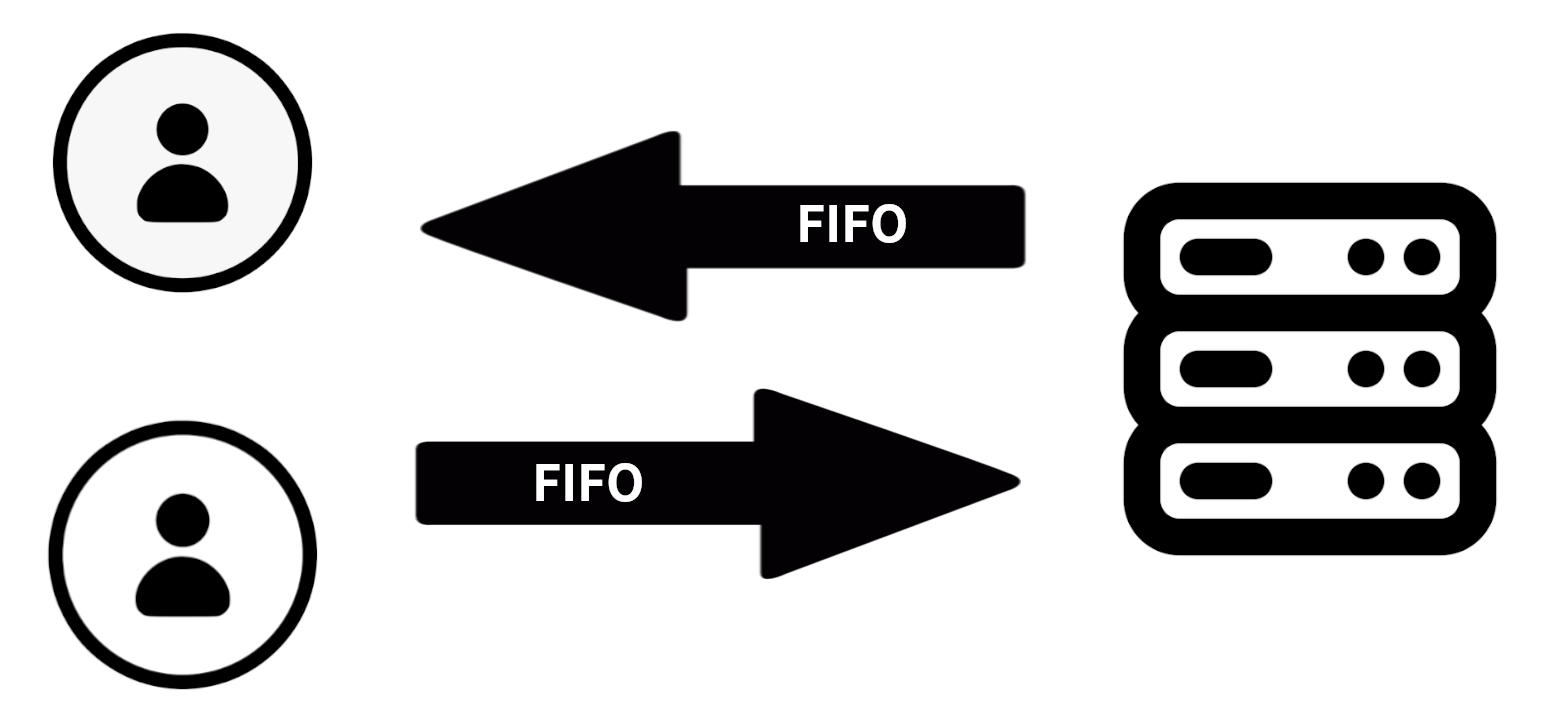
\includegraphics{images/arq1.png}
            \caption*{Figura 1. Primeira arquitetura idealizada}
            \label{fig:Arq1}
        \end{figure}

        Apesar de o servidor não precisar de saber necessariamente qual dos clientes está a comunicar consigo, o contrário não acontece. Por exemplo, vamos supor que dois clientes enviam uma mensagem em simultâneo ao servidor, como as mensagens são diferentes é expectável que os clientes recebem respostas diferentes.

        Contudo, após enviarem as mensagens, os dois clientes vão tentar ler do mesmo FIFO, e nada impede que a mensagem destinada a um cliente seja lida pelo outro e vice-versa. 


    \section{FIFOs Separados}

        A única forma de assegurar que cada cliente lê apenas a mensagem que lhe é destinada, reside na criação de canais de comunicação separados.

        \newpage

        \begin{figure}[hb!]
            \centering
            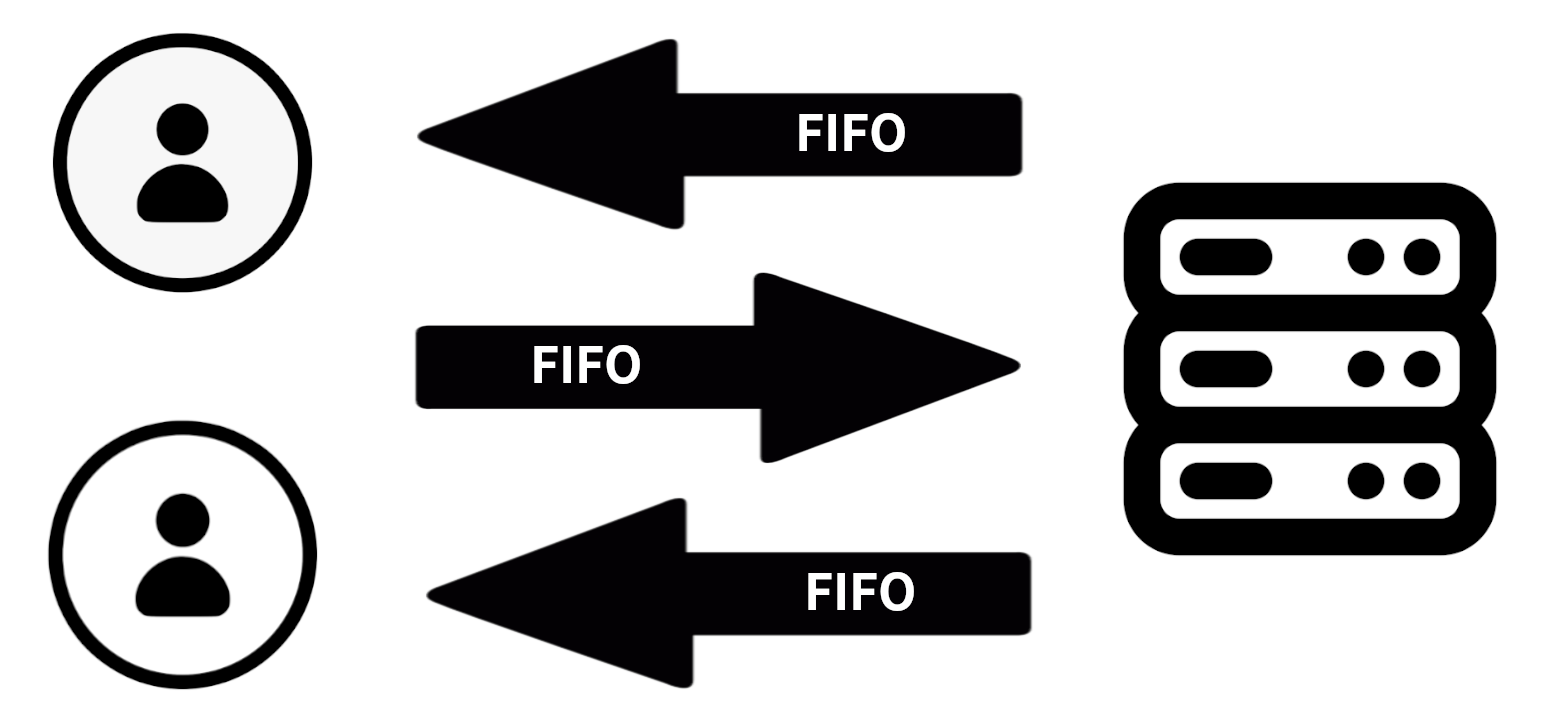
\includegraphics{images/arq2.png}
            \caption*{Figura 2. Arquitetura final}
            \label{fig:Arq2}
        \end{figure}

        Nesta conceção de canais separados, um cliente é responsável por criar o FIFO que mais tarde o servidor deverá utilizar para encaminhar as mensagens destinadas a esse mesmo cliente, pelo que nunca haverá qualquer interferência entre clientes.

        Após o comunicação terminar, o FIFO deixa de ser necessário e como tal também cabe ao cliente assegura que o mesmo é eliminado, garantindo que os outros clientes terão espaço para criar os seus FIFOs.


    \section{Protocolo}

        Com a existência de tantos FIFOs torna-se insustentável ler $X$ \textit{bytes} de um canal e $Y$ de outro qualquer, é muito mais viável definir um protocolo no qual apenas determinadas estruturas de dados passam pelos FIFOs.

        \begin{wrapfigure}{r}{0.4\textwidth}
            \begin{center}
                \vspace{-22pt}
                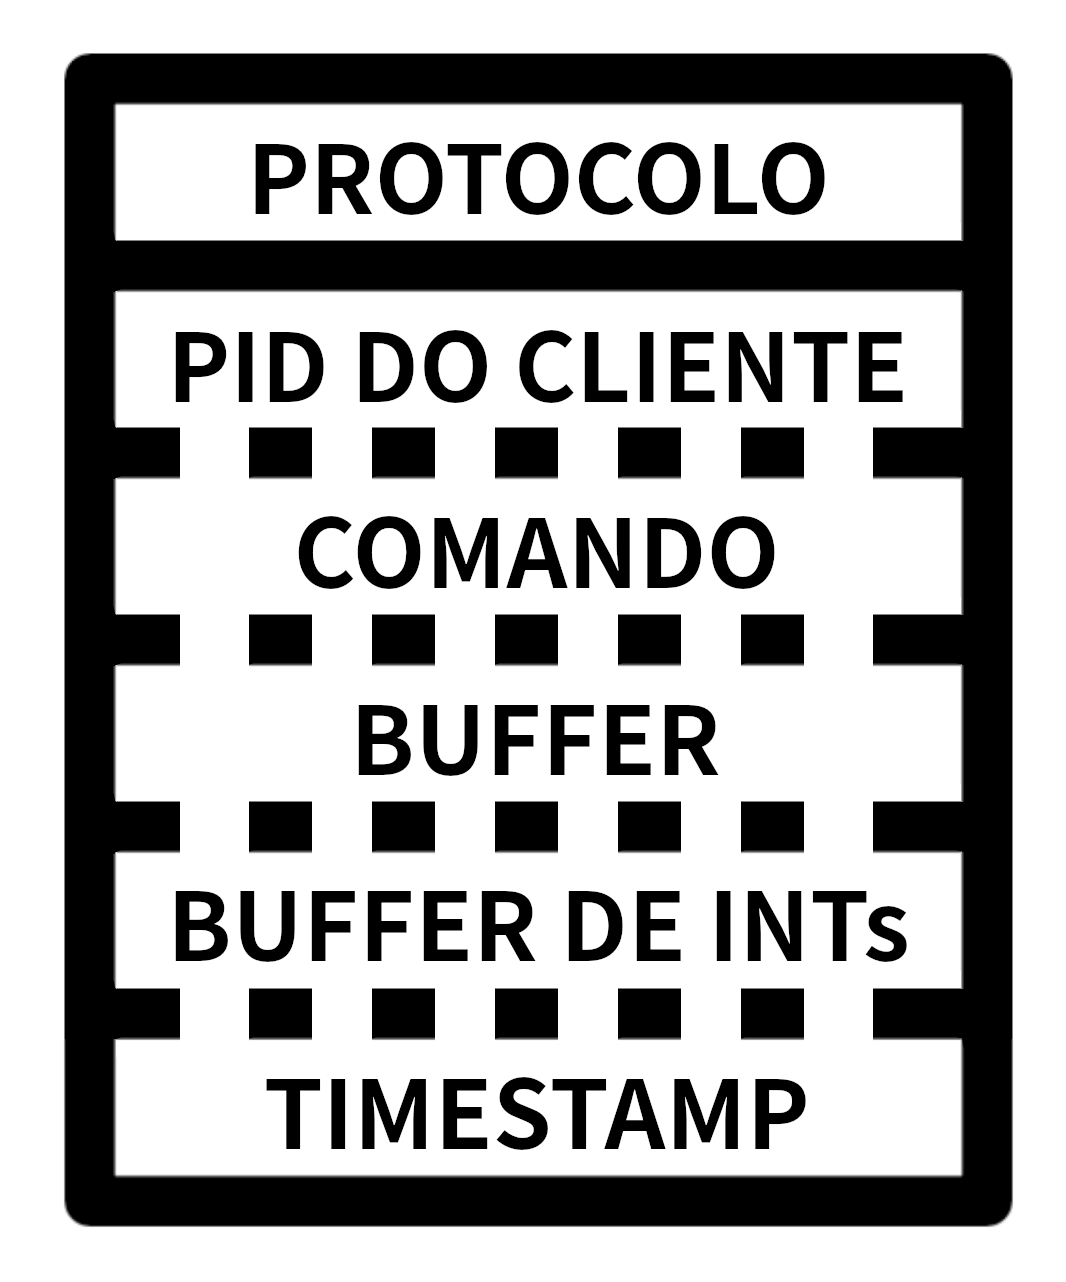
\includegraphics[width=0.3\textwidth]{images/protocol.png}
                \caption*{Figura 3. Estrutura do pacote}
                \vspace{-30pt}
            \end{center}
        \end{wrapfigure}

        Este pacote é a única estrutura de dados transmitida, assim tanto os clientes como o servidor vão sempre estar à espera um tamanho fixo de \textit{bytes}.

        Por exemplo, caso seja necessário transmitir um inteiro que represente o tempo de execução de um programa, esse inteiro terá de ser inserido num pacote (no campo \textit{timestamp}), já que as leituras e escritas estão programadas para $X$ \textit{bytes} (tamanho do pacote).


\chapter{Funcionalidades}

    O cliente tem ao seu dispor várias funcionalidades das quais pode tirar partido, sendo que umas são direcionadas para CPU (execução de programas), enquanto que outras priorizam o acesso a memória e a disco (consulta de programas).

    \section{Execução Única}

        \begin{wrapfigure}{r}{0.4\textwidth}
            \begin{center}
                \vspace{-22pt}
                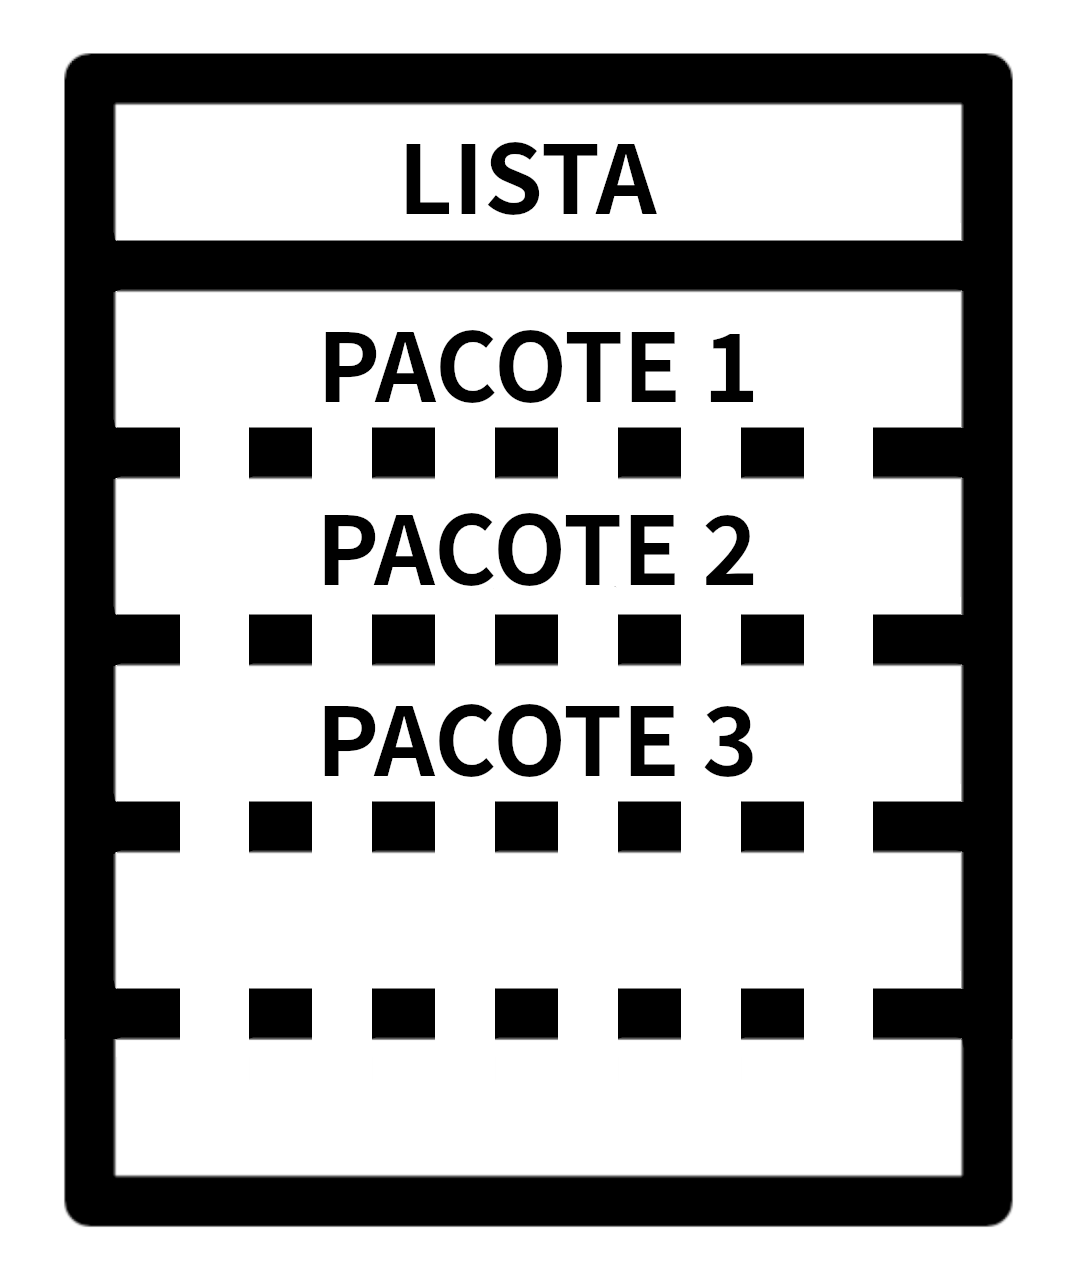
\includegraphics[width=0.3\textwidth]{images/list.png}
                \caption*{Figura 4. Lista de pacotes}
                \vspace{-30pt}
            \end{center}
        \end{wrapfigure}

        Esta funcionalidade foi bastante fácil de implementar na perspetiva do cliente, basta criar um processo filho para executar o programa desejado e fazer o processo pai esperar até que este termine, obtendo assim o tempo de execução.

        Contudo, como o servidor tem de responder a outras funcionalidades, é necessário seguir a seguinte abordagem e criar uma lista com os clientes ativos.

        \begin{figure}[hb!]
            \centering
            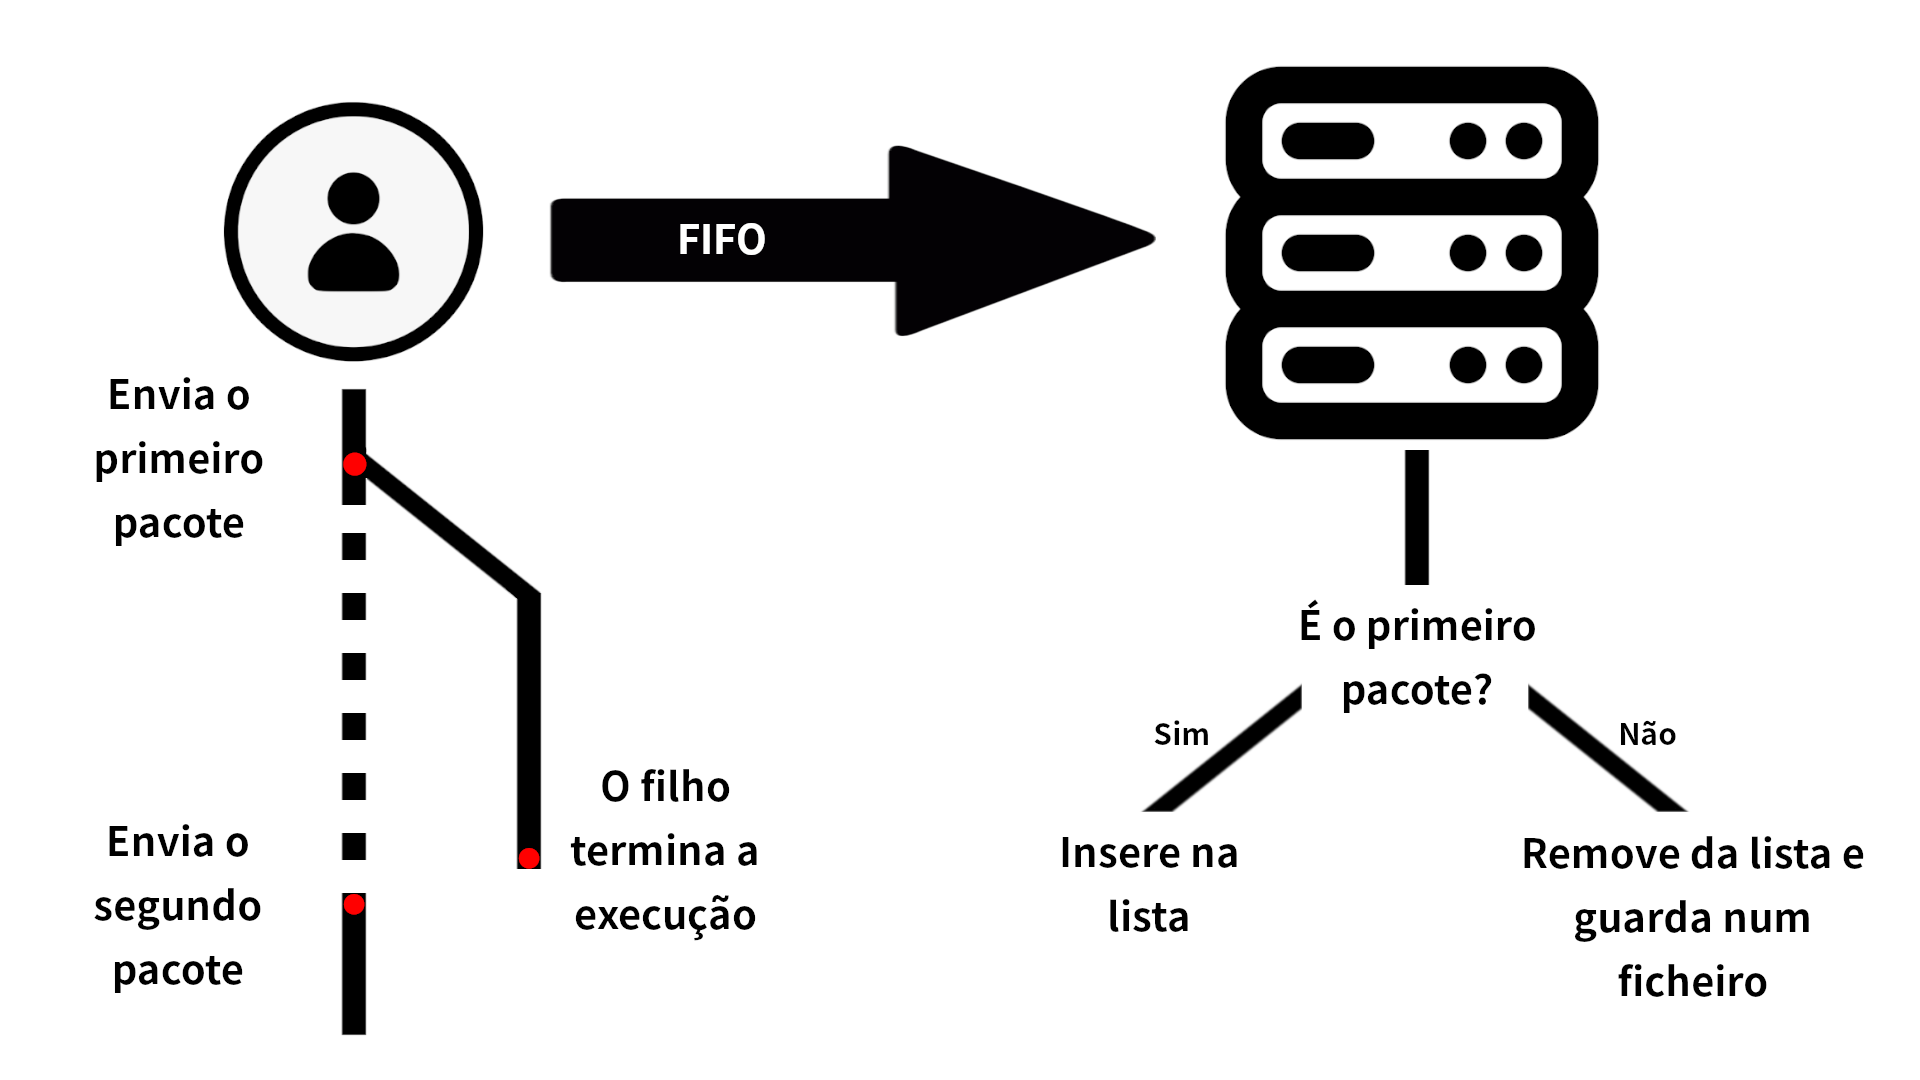
\includegraphics[width=0.8\textwidth]{images/uniq.png}
            \caption*{Figura 5. Esquema da funcionalidade}
            \label{fig:Uniq}
        \end{figure}

        \begin{enumerate}
            \item Antes de criar um filho, o cliente envia um pacote com informações de estado.
            \item O servidor armazena o pacote numa lista dinâmica e aguarda nova comunicação.
            \item Após o filho do cliente terminar a sua execução, é gerado e enviado outro pacote.
            \item Através do \textit{pid}, o servidor sabe que é a segunda vez que o cliente envia um pacote, o que significa que execução terminou.
            \item O pacote é removido da lista e guardado num ficheiro.
        \end{enumerate}

    \section{Execução Encadeada}

        O objetivo desta funcionalidade consiste em reproduzir o operador de \textit{pipeline} presente nos sistemas UNIX, de facto esta foi a parte mais desafiante do trabalho.

        A interação entre o cliente e o servidor realiza-se da mesma forma que numa execução única, contudo terão de ser criados tantos filhos como programas a executar dentro do \textit{pipeline}.

        Como não sabemos à partida quantos \textit{pipes} serão necessários, optámos por declarar $64$, podíamos ter utilizado uma alocação dinâmica, contudo parece-nos que $64$ \textit{pipes} é um número mais que suficiente para além de não representar um grande peso para a \textit{stack}.

        Para que o \textit{pipeline} funcione, os \textit{inputs} e \textit{outputs} dos programas têm de ser redirecionados devidamente, assim o STDOUT\_FILENO foi redirecionado para a ponta de escrita do \textit{pipe} atual, enquanto que o STDIN\_FILENO foi redirecionado para a ponta de leitura do \textit{pipe} anterior.

        \begin{figure}[hb!]
            \centering
            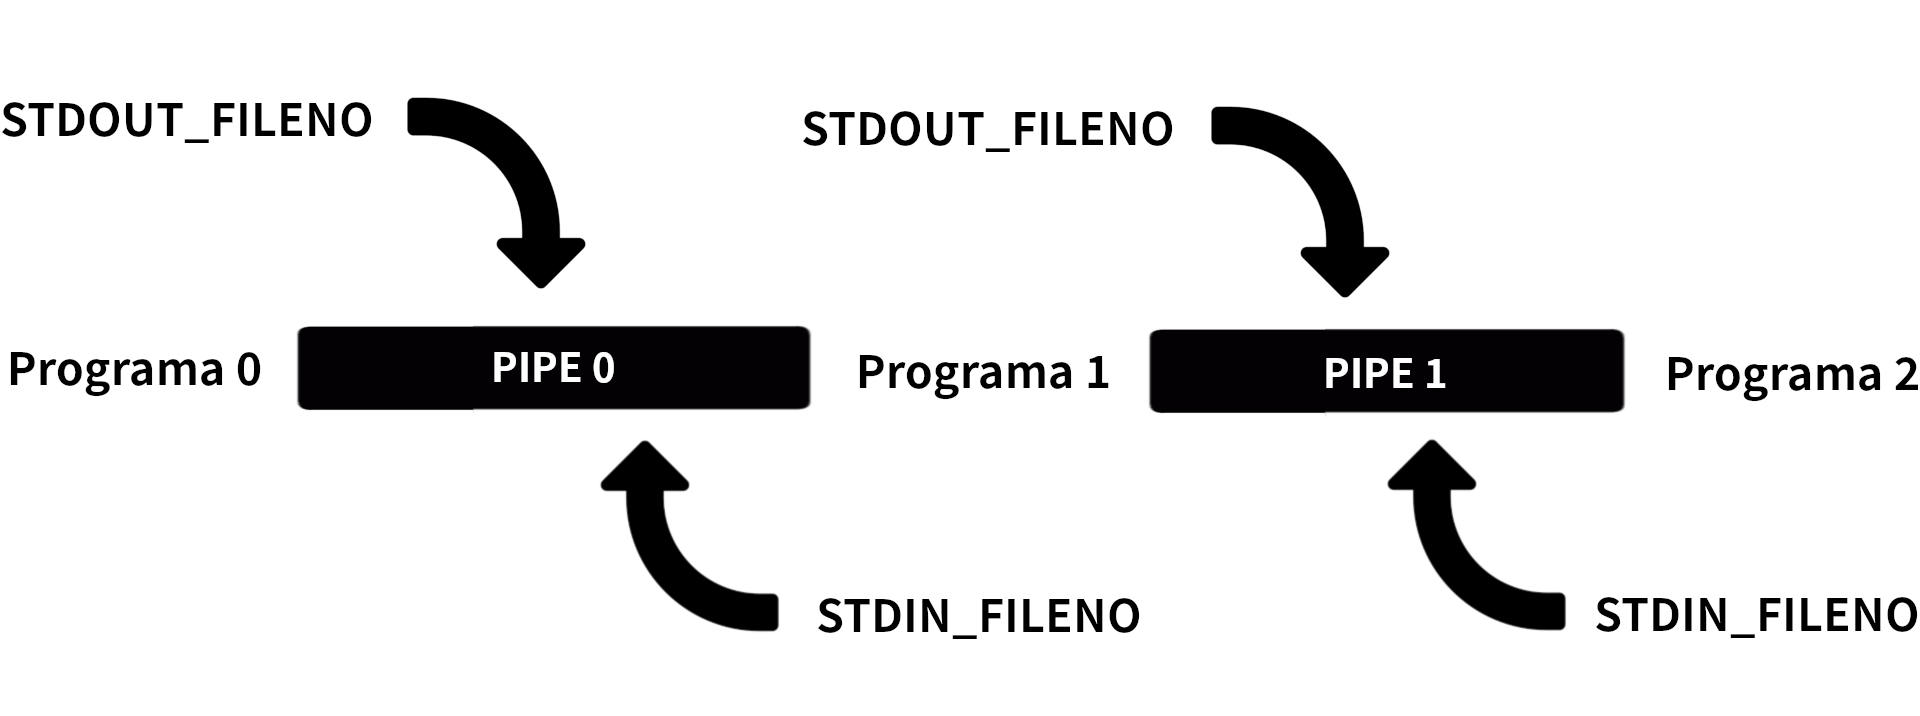
\includegraphics[width=0.85\textwidth]{images/pipeline.png}
            \caption*{Figura 6. Esquema do \textit{pipeline}}
            \label{fig:PIPE}
        \end{figure}

        É verdade que o \textit{standard input} e \textit{output} estão constantemente a ser redirecionados pelos filhos do cliente, contudo à que ter em atenção que o STDIN\_FILENO do programa $0$ não pode ser modificado, bem como o STDOUT\_FILENO do último programa, neste caso o programa 2.

    \section{Consulta de Programas em Execução}

        Ao contrário das funcionalidades anteriores, nas quais somente o cliente enviava pacotes, esta funcionalidade requer troca de informação de ambos os lados, pelo que os FIFOs extra apenas serão criados por clientes que decidam usufruir deste tipo de funcionalidades.

        Como os programas em execução são guardados pelo servidor na sua lista de pacotes, podemos guiar-nos pela seguinte metodologia.

        \begin{enumerate}
            \item O cliente cria um FIFO ao qual atribui um nome que corresponde ao seu \textit{pid.}
            \item É criado um pacote com informações de estado e enviado pelo FIFO permanente.
            \item O servidor recebe o pacote e obtém o \textit{pid} presente no mesmo.
            \item O FIFO é aberto pelo servidor que por sua vez envia uma cópia dos pacotes presentes na lista de pacotes.
            \item À medida que o cliente recebe os pacotes, imprime no \textit{standard output} parte da informação contida nos mesmos.
            \item Assim que o cliente lê um EOF, o descritor de leitura é fechado e o FIFO é eliminado.
        \end{enumerate}

    \section{Consulta de Programas Terminados}

        Esta funcionalidade é muito parecida à anterior, contudo, uma vez que os programas a consultar já terminaram, isso significa que temos de aceder aos ficheiros e não à lista, o que é significativamente mais lento, visto que os ficheiros estão em disco, ao passo que a lista está em memória.

        Tendo este pormenor em conta, o servidor é responsável por criar vários filhos que irão aceder aos ficheiros e ler os respetivos pacotes. Depois de efetuarem a leitura, a informação é transmitida ao processo pai através de \textit{pipes} anónimos e é feito um tratamento dos dados conforme o comando invocado pelo cliente.

        De resto, a interação entre o servidor e o cliente é bastante semelhante à mencionada anteriormente.

        
\chapter{Decisões Tomadas}

    Durante a realização do trabalho prático deparámo-nos imensas vezes com situações nas quais as decisões tomadas não foram de todo consensuais.

    \begin{itemize}
        \item\large Input \\ \normalsize Quando um cliente pretende executar um programa ou uma série de programas encadeados, o \textit{input} é passado entre aspas, como não sabemos \textit{a priori} qual será o tamanho do mesmo, definimos que o seu tamanho máximo seria de $2048$ \textit{bytes.} 

        \item\large Pacote \\ \normalsize Os \textit{buffers} presentes nos pacotes não podem ser alocados dinamicamente, têm de ser estáticos, caso contrário as transmissões de pacotes através dos FIFOs seriam inúteis, visto que estariam a ser escritos/lidos endereços de memória e não o seu conteúdo.   

        \item\large Pipeline \\ \normalsize Tal como foi mencionado anteriormente, apenas é possível declarar $64$ \textit{pipes}, pelo que uma sequência de programas encadeados executará no máximo $65$ programas.  

        \item\large Chunck Size \\ \normalsize Quando um cliente pretende consultar programas terminados, cada um dos processos filhos do servidor é responsável por ler um determinado número de ficheiros, como criar processos e ler ficheiros são operações bastante demoradas, pensámos que cada filho deveria ler no máximo $5$ ficheiros (é apenas um palpite).
    \end{itemize}


    Grande parte destes problemas poderiam ser resolvidos através da alocação dinâmica de memória, contudo não optámos por seguir esse caminho uma vez que seria muito difícil evitar \textit{memory leaks}, visto que no momento de criação de um processo filho o espaço de endereçamento do processo pai é copiado \textit{(copy-on-write)}. E tendo filhos que por sua vez criam mais filhos, muito dificilmente seriamos capazes de libertar toda a memória alocada. 


\chapter{Conclusão}

    Durante a realização deste trabalho prático enfrentámos vários desafios que nos obrigaram a pensar e refletir qual seria a melhor estratégia a adotar. Nunca vimos estas dificuldades como algo maçador, muito pelo contrário, procurámos sempre dar o nosso e seguir em frente a fim de apresentar um projeto do qual nos pudéssemos orgulhar.

    Desta forma, acreditamos que cumprimos com o nosso objetivo, para além de termos implementado devidamente as funcionalidades básicas, as funcionalidades avançadas também apresentam o comportamento esperado.

    É certo que podíamos ter feito algumas alterações que certamente melhorariam o projeto, porém só em casos muito excecionais é que o nosso programa vai falhar.

    Em suma, foi bastante gratificante ver na prática como as chamadas ao sistema apresentadas nas aulas podem ser ajustadas de forma a criar interações entre vários clientes e um servidor, o que também serviu para consolidar alguns conceitos que ficaram pouco claros numa primeira abordagem.

\end{document}